%Paqueterias
\documentclass[12pt,letterpaper,final]{article}%Tipo de documento
\usepackage[utf8]{inputenc}
\usepackage[spanish,es-nodecimaldot,es-tabla]{babel}
\usepackage{amsmath}
\usepackage{amssymb}
\usepackage{graphicx}
\usepackage[left=2cm,right=2cm,top=2cm,bottom=2cm]{geometry}
\usepackage{titlesec}
\usepackage{hyperref}
\usepackage{pdflscape}
\usepackage{gensymb}
\usepackage{stix2}
\usepackage{siunitx}
\usepackage{tikz}
\usepackage[backend=bibtex,style=ieee]{biblatex}
\addbibresource{refer_repo_6_rev.bib}
\graphicspath{{img/}}
\baselinestretch
\renewcommand{\baselinestretch}{1.25}%Comando de interlineado
%%%%%%%%%%%%%%%%%%%%%
\usepackage{fancyhdr}%Encabezados
\pagestyle{fancy}
\fancyhf{}
\lhead[\leftmark]{Revisión}
\rhead[]{\rightmark}
\lfoot[\thepage]{}
\rfoot[]{\thepage}
\renewcommand{\headrulewidth}{0.5pt}
\renewcommand{\footrulewidth}{0pt}
\fancypagestyle{plain}{
	\fancyhead[L]{Omar Arturo Castillo M\'endez}
	\fancyfoot[R]{\thepage}
	\renewcommand{\headrulewidth}{0.4pt}
	\renewcommand{\footrulewidth}{0.4pt}
}
\pagestyle{fancy}
%%%%%%%%%%%%%%%%%%%%%%%%%
%Datos del documento
\title{Reporte }
\date{}
\author{M.I.E. Omar Arturo Castillo M\'endez}
\begin{document}
	%%%%%%%%%%%%%%%%%%%%%%%%%%%%%%%%%%%%%%%%%%%%%%%%%%%%%
	\begin{titlepage}%Portada
		\centering
		
\includegraphics[scale=1]{logo}
		\vspace{0.1cm}
		{\bfseries\LARGE Tecnol\'ogico Nacional de M\'exico \par}
		{\bfseries\LARGE Centro Nacional de Investigaci\'on y Desarrollo Tecnol\'ogico \par}
		\vspace{0.25cm}
		{\scshape\Large Departamento de Ciencias en Ingenier\'ia Electr\'onica \par}
		\vspace{0.25cm}
		{\scshape\Large Diseño, construcci\'on y puesta en marcha de un regenerador de energ\'ia para el desarrollo y la validaci\'on de estrategias de modelado matem\'atico \par}
		\vspace{0.25cm}
		{\itshape\Large Revisión  \par}
		\vspace{0.25cm}
		{\bfseries Director de tesis: \par}
		\vspace{0.2cm}
		{Dr. V\'ictor Manuel Alvarado Mart\'inez \par}
		\vspace{0.2cm}
		{\bfseries Co-Directora de tesis: \par}
		\vspace{0.2cm}
		{Dra. Maria Guadalupe L\'opez L\'opez \par}
		\vspace{0.2cm}
		{\bfseries Comit\'e revisor: \par}
		\vspace{0.2cm}
		{Dr. Jos\'e Francisco G\'omez Aguilar \par}
		\vspace{0.2cm}
		{Dr. Ricardo Fabricio Escobar Jim\'enez  \par}
		\vspace{0.2cm}
		{Dr. Jarniel Garc\'ia Morales \par}
		\vspace{0.2cm}
		{\bfseries Presenta: \par}
		{M.I.E. Omar Arturo Castillo M\'endez \par}
		\vspace{0.2cm}
		{\today \par}
	\end{titlepage}
	%%%%%%%%%%%%%%%%%%%%%%%%%%%%%%%%%%%%%%%%%%%%%%%%%%%%%%%
	%\tableofcontents{\thispagestyle{empty}}
	%\tableofcontents{\thispagestyle{empty}} Pagina sin numeracion
	\newpage
	%\listoffigures{\thispagestyle{empty}}
	%\newpage
	\setcounter{page}{1}
%------------------------------------------------------------------------%
%-----------------------AQUI COMIENZA EL DOCUMENTO-----------------------%
\section{Modelo}
\subsection{Modelo: Kilkovsky}
\textbf{Consideraciones del modelo}
\begin{itemize}
	\item Los coeficientes de transferencia de calor y las propiedades térmicas de la masa de almacenamiento de calor y del gas no varían a lo largo de un período.
	\item Los coeficientes de transferencia de calor y las propiedades térmicas de la masa de almacenamiento de calor y del gas no varían a lo largo de un período
	y son idénticos en todas las partes del regenerador en ese período.
	\item Se desprecia la conductividad térmica longitudinal.
	\item Las temperaturas del gas de entrada en ambos periodos permanecen constantes.
	Los caudales másicos de los gases de calefacción y refrigeración no varían a lo largo de cada período.
	La transferencia de calor entre el gas y el sólido puede representarse en términos de un coeficiente global de transferencia de calor
	que relaciona la temperatura del gas con la temperatura media del sólido. Además, la tasa de transferencia de calor
	en el lecho compacto a cualquier altura está representada por la variación temporal de la temperatura media del sólido
	.
	La capacidad calorífica del gas en los canales del lecho compacto en cualquier instante es pequeña en relación con
	la capacidad calorífica del sólido y, por lo tanto, puede despreciarse.
	
\end{itemize}
La ecuación para el solido es la siguiente:
\begin{equation}
	M_bC_{p,b}\frac{\partial T_s}{\partial t} = hA(T_g - T_s)
\end{equation}
La ecuación para la fase del gas:
\begin{equation}
	m_gC_{p,g}L \frac{\partial T_g}{\partial x} + M_gC_{p,g}\frac{\partial T_g}{\partial t} = hA(T_s - T_g)
\end{equation}

\begin{table}[ht!]
	\begin{center}
		\begin{tabular}{|c|c|c|}
			\hline
			\multicolumn{2}{ |c|}{Datos del modelo:Variables} & unidades \\ \hline
			$T_s$ & Temperatura del lecho & $^\circ C$ \\ 
			$T_g$ &  Temperatura del gas & $^\circ C$ \\ \hline
			\multicolumn{2}{ |c|}{Datos del modelo: Constantes} & unidades \\ \hline
			$T_0$ & Temperatura inicial del lecho & $^\circ C$ \\
			$T_{en}$ & Temperatura de entrada & $^\circ C$ \\
			$\rho_s$ & Densidad del lecho & $kg/m^3$ \\
			$\epsilon_s$ & porosidad del lecho & $kg/m^3$ \\
			$K_{s,x}$&  Conductividad térmica efectiva del solido & $W \cdot m^{-1} \cdot K^{-1} $ \\
			$K_{a,x}$&  Conductividad térmica efectiva del gas & $W \cdot m^{-1} \cdot K^{-1} $ \\
			$h$ & Coeficiente de transferencia de calor & $W \cdot m^{-2} \cdot K^{-1}$ \\
			$a_p$ & Área superficial de las partículas por unidad de volumen & $m^2$ \\
			$u$ & Velocidad del flujo &  $m \cdot s^{-1}$  \\
			$C_{p,s}$&  Calor específico del lecho & $J \cdot kg^{-1} \cdot K^{-1}$\\
			$C_{p,g}$&  Calor específico del gas & $J \cdot kg^{-1} \cdot K^{-1}$\\
			\hline
			
			
		\end{tabular}
	\end{center}
\end{table}
\newpage
\textbf{Condiciones iniciales y de frontera}
\newline
Al inicio del proceso de calentamiento, la temperatura del lecho es igual a la temperatura ambiente:
\newline
\begin{center}
	$T_s = T_{amb}$; en $t=0$	
\end{center}
En cuanto a las condiciones de frontera, en la entrada del lecho la temperatura del gas:
\begin{center}
	$T_g = T_{en}$; en $x=0$
\end{center} 
La condición de frontera del solido anterior a la entrada no hay lecho, por lo tanto:
\begin{center}
	$\frac{\partial T_s}{\partial x} = 0$; en $x=0$
\end{center}
Para la salida del lecho tanto para el gas como en el lecho, ya no se puede intercambiar mas calor:
\begin{center}
	$\frac{\partial T_s}{\partial x} = 0$; en $x=L$
\end{center}
\begin{center}
	$\frac{\partial T_g}{\partial x} = 0$; en $x=L$
\end{center}

Los parámetros del modelo son los siguientes:
\begin{table}[ht!]
	\begin{center}
		\caption{Propiedades del gas: Aire}
		\begin{tabular}{|c|c|c|c|}
			\hline
			\multicolumn{2}{ |c|}{Propiedades del gas} &  & unidades \\ \hline
			$T_0$ & Temperatura inicial del gas & 25 & $^\circ C$ \\
			$T_en$ & Temperatura de entrada & 727& $^\circ C$ \\
			$\rho_g$ & Densidad del gas &0.51 &$kg \cdot m^{-3}$ \\
			$h$ & Coeficiente de transferencia de calor &354.4538 & $W \cdot m^{-2} \cdot K^{-1}$ \\
			$u$ & Velocidad superficial del gas &3.6 & $m \cdot s^{-1}$  \\
			$C_{p,g}$&  Calor específico del gas & 1012 & $J \cdot kg^{-1} \cdot K^{-1}$\\
			\hline	
		\end{tabular}
	\end{center}
\end{table}

\begin{table}[ht!]
	\begin{center}
		\caption{Propiedades del lecho usado como en el regenerador}
		\begin{tabular}{|c|c|c|c|}
			\hline
			\multicolumn{2}{ |c|}{Propiedades del lecho} &  & unidades \\ \hline
			$T_0$ & Temperatura inicial del lecho & 25 & $^\circ C$ \\
			$\rho_s$ & Densidad del lecho &3970 &$kg \cdot m^{-3}$ \\
			$\epsilon_s$ & Porosidad del lecho &0.38 &  \\
			$h$ & Coeficiente de transferencia de calor &354.4538 & $W \cdot m^{-2} \cdot K^{-1}$ \\
			$a_p$ & Área superficial de las partículas por unidad de volumen &124& $m^{-1}$ \\
			$C_{p,s}$&  Calor específico del lecho & 765 & $J \cdot kg^{-1} \cdot K^{-1}$\\
			\hline			
		\end{tabular}
	\end{center}
\end{table}

\begin{table}[ht!]
	\begin{center}
		\caption{Resultados obtenidos a partir de las características del gas y del lecho}
		\begin{tabular}{|c|c|c|c|}
			\hline
			\multicolumn{2}{ |c|}{Parámetros calculados} &  & unidades \\ \hline
			$K_{s,x}$&  Conductividad térmica efectiva del solido & 1.4497& $W \cdot m^{-1} \cdot K^{-1} $ \\
			$K_{a,x}$&  Conductividad térmica efectiva del gas &0.03808 &$W \cdot m^{-1} \cdot K^{-1} $ \\
			$h$ & Coeficiente de transferencia de calor & 92.7 & $W \cdot m^{-2} \cdot K^{-1}$ \\
			$St$&  Stanton & 5.906 & \\
			$Bi$&  Biot & 0.088 & \\
			$Pr$&  Prandlt & 0.7 & \\
			$Pr$&  Nusselt & 134.1842 & \\
			$Re_d$&  Reynolds intersticial & 1513.1868 & \\
			\hline			
		\end{tabular}
	\end{center}
\end{table}
\newpage
\subsection{Análisis hidráulico}
Se elaboró el siguiente análisis con la finalidad de visualizar la región de operación del regenerador. Así mismo, se tomó en cuenta una longitud del lecho, diámetro de partícula y velocidades del aire variables, para observar como serian sus efectos en el numero de Reynolds del lecho, caídas de presión, el numero de Stanton y Biot.
\begin{table}
	\begin{center}
		\caption{Rango de propiedades para el análisis hidráulico}
		\begin{tabular}{|c|c|c|}
			\hline
			\multicolumn{2}{ |c|}{Parámetro } & unidades \\ \hline
			Longitud del lecho & 0.3 - 2& $m $ \\
			Velocidad superficial &1.5 - 5 &$m \cdot s^{-1} $ \\
			Diámetro de partícula & 0.5 - 5  & $m $ \\
			\hline			
		\end{tabular}
	\end{center}
\end{table}
\subsubsection{Numero de Reynolds}
Para obtener este parámetro adimensional se obtuvo mediante la siguiente formula:
\begin{equation}\label{Ecu_reynolds}
	Re = \frac{d_p U_s \rho}{\mu}
\end{equation}
Donde $d_p$ corresponde al diámetro de partícula, $U_s$ a la velocidad superficial, $\rho$ a la densidad del gas y $\mu$ a la viscosidad dinámica del aire
\begin{figure}[ht!]\label{Reynolds_vs_Us}
	\centering
	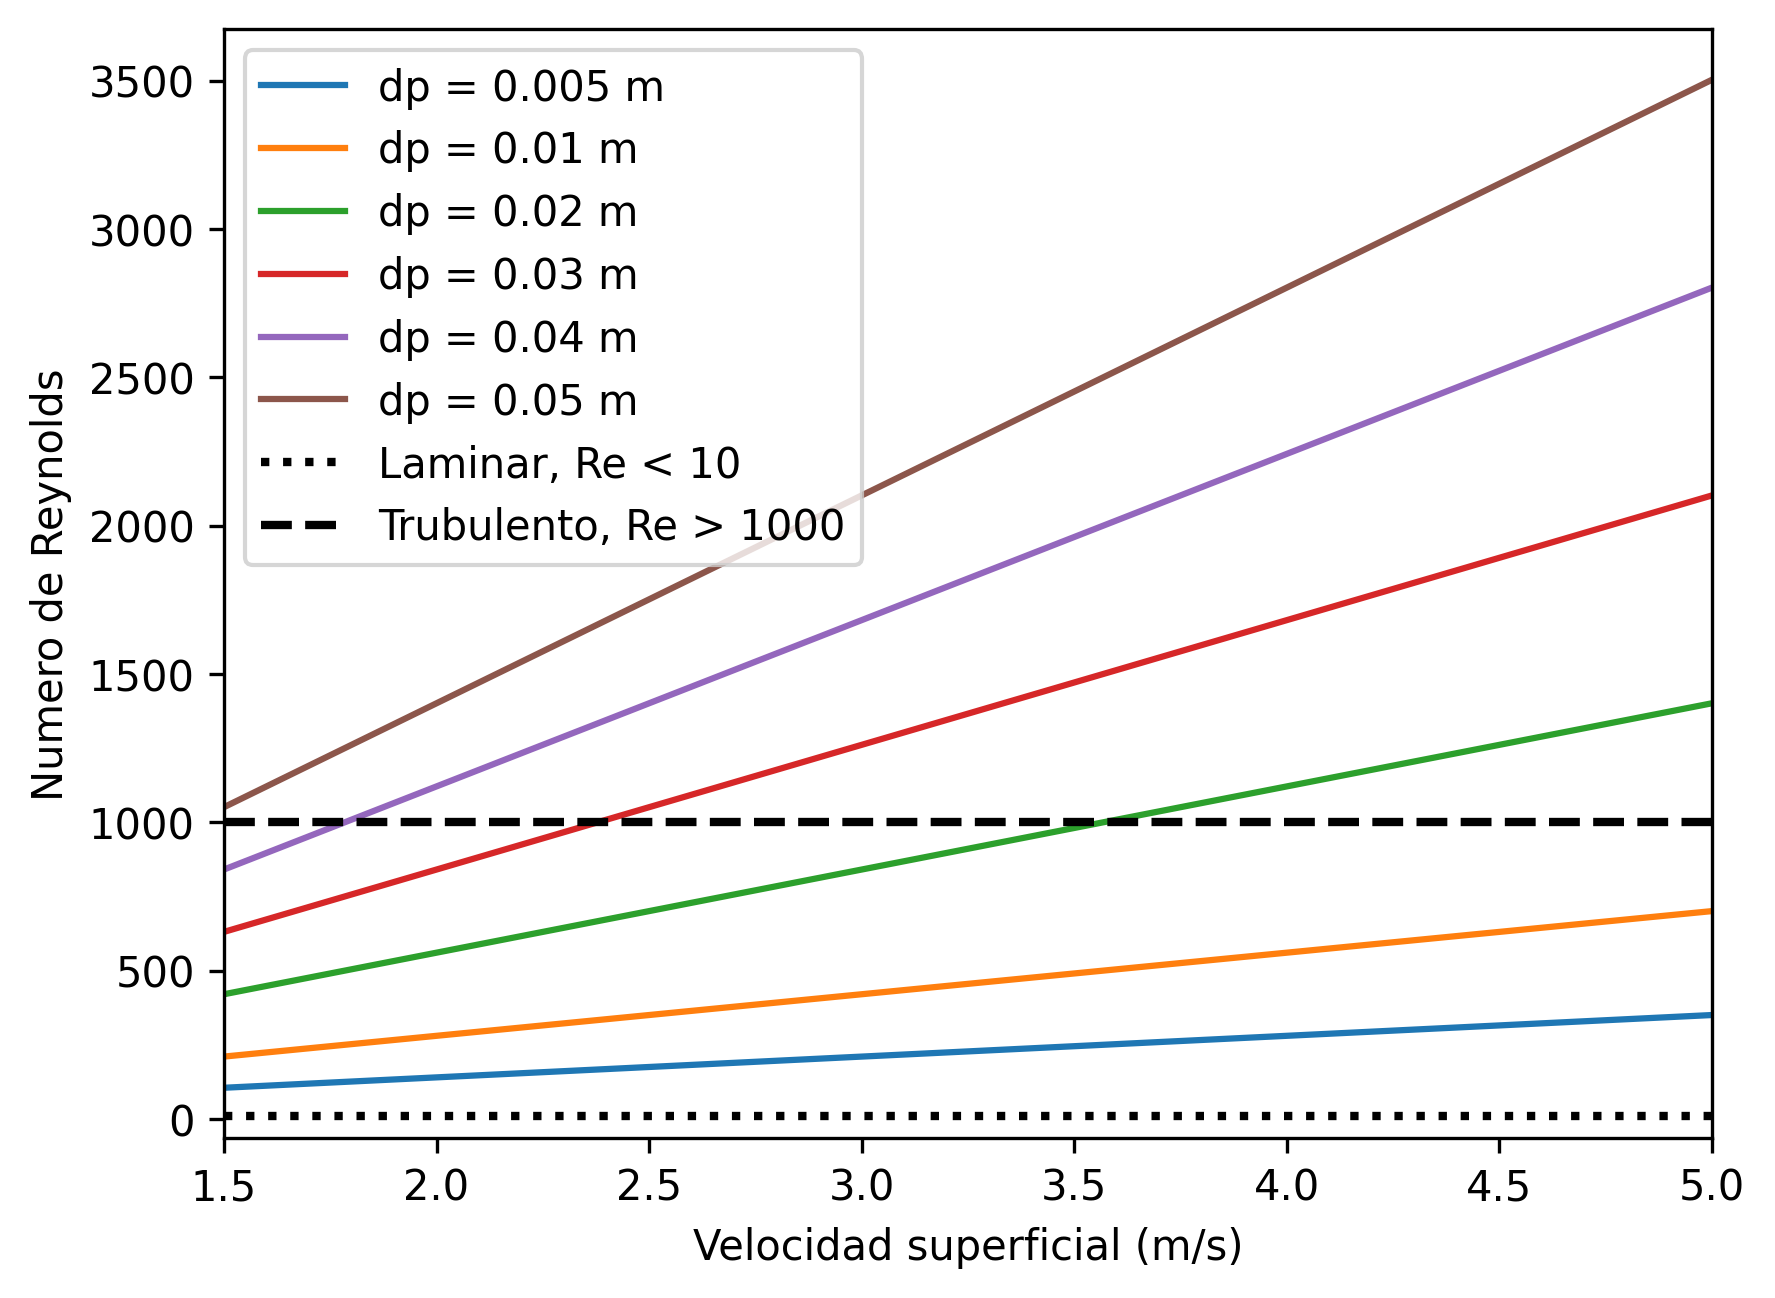
\includegraphics[scale=.9]{RevsUs.png}
	\caption{Efecto de la velocidad superficial en el numero de Reynolds}
\end{figure}
\newline
En la imagen anterior, se muestra como es el cambio del numero de Reynolds para el rango de velocidades y de igual manera el efecto del diámetro de partícula. Para lechos empacados el flujo laminar esta representado para números menores a $Re<10$, transitorio entre $10<Re<1000$ y turbulento para $Re>1000$.
En la siguiente imagen, se graficó respecto al tamaño de la partícula para visualizar el cambio desde esa perspectiva. 
\begin{figure}[ht!]\label{Reynolds_vs_Dp}
	\centering
	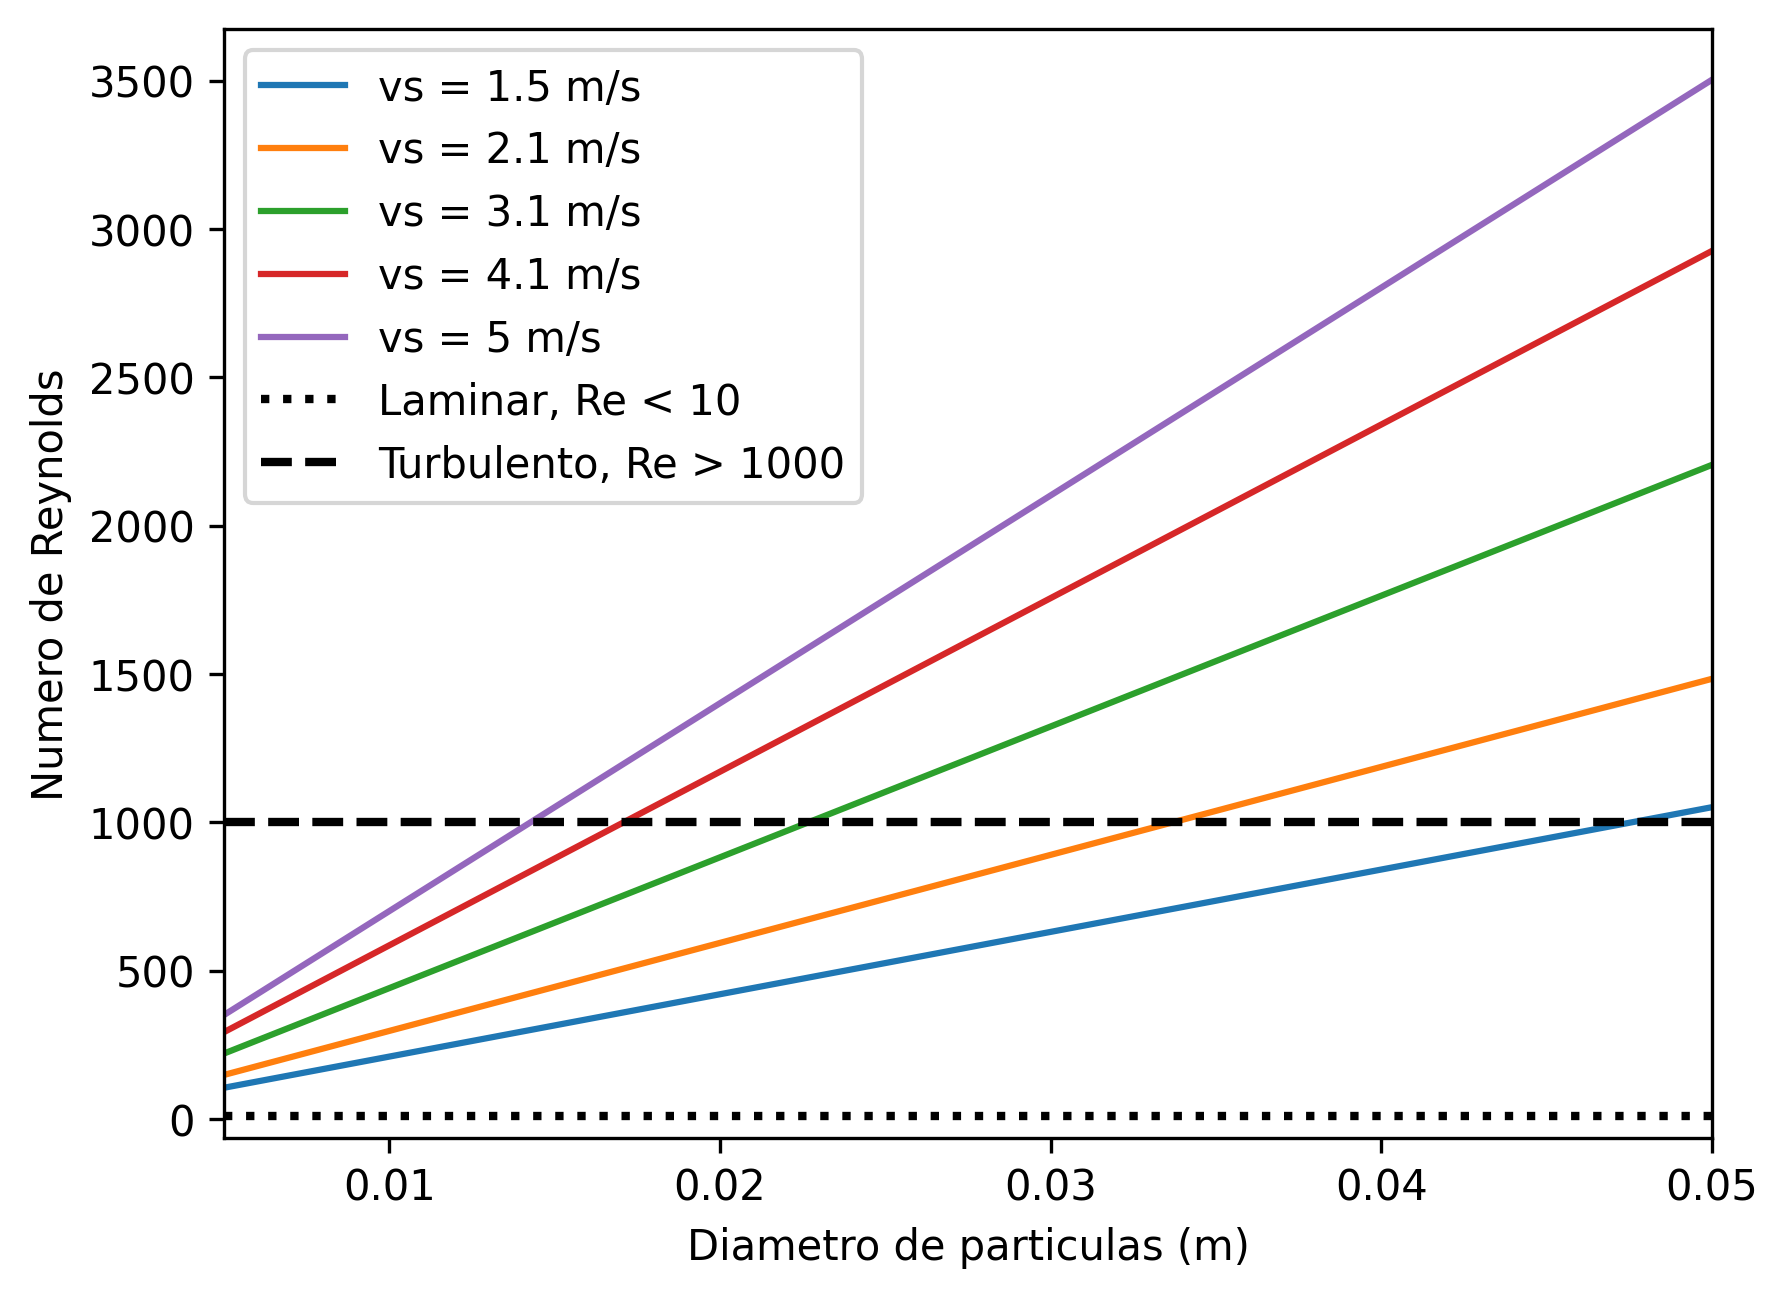
\includegraphics[scale=0.9]{RevsDp.png}
	\caption{Efecto del diámetro de partícula en el numero de Reynolds}
\end{figure}
\subsubsection{Caída de presión}
La diferencia de presión a lo largo del regenerador se obtuvo mediante la siguiente relación\cite{Valle-Guadarrama2015}:
\begin{equation}\label{Ecu_ergun}
	\Delta p = [ \frac{150}{Re} + 1.75 ] [ \frac{(U_s \rho)^2 L (1-\epsilon)}{\rho d_p \epsilon^3}  ]
\end{equation}
Donde $Re$ es el numero de Reynolds, $U_s$ velocidad superficial, $\rho$ la densidad del gas, $L$ longitud del lecho en metros, $\epsilon$ corresponde a la porosidad del lecho y $d_p$ el diámetro de la partícula del lecho.
\begin{figure}\label{CaidaP_por_dp}
	\centering
	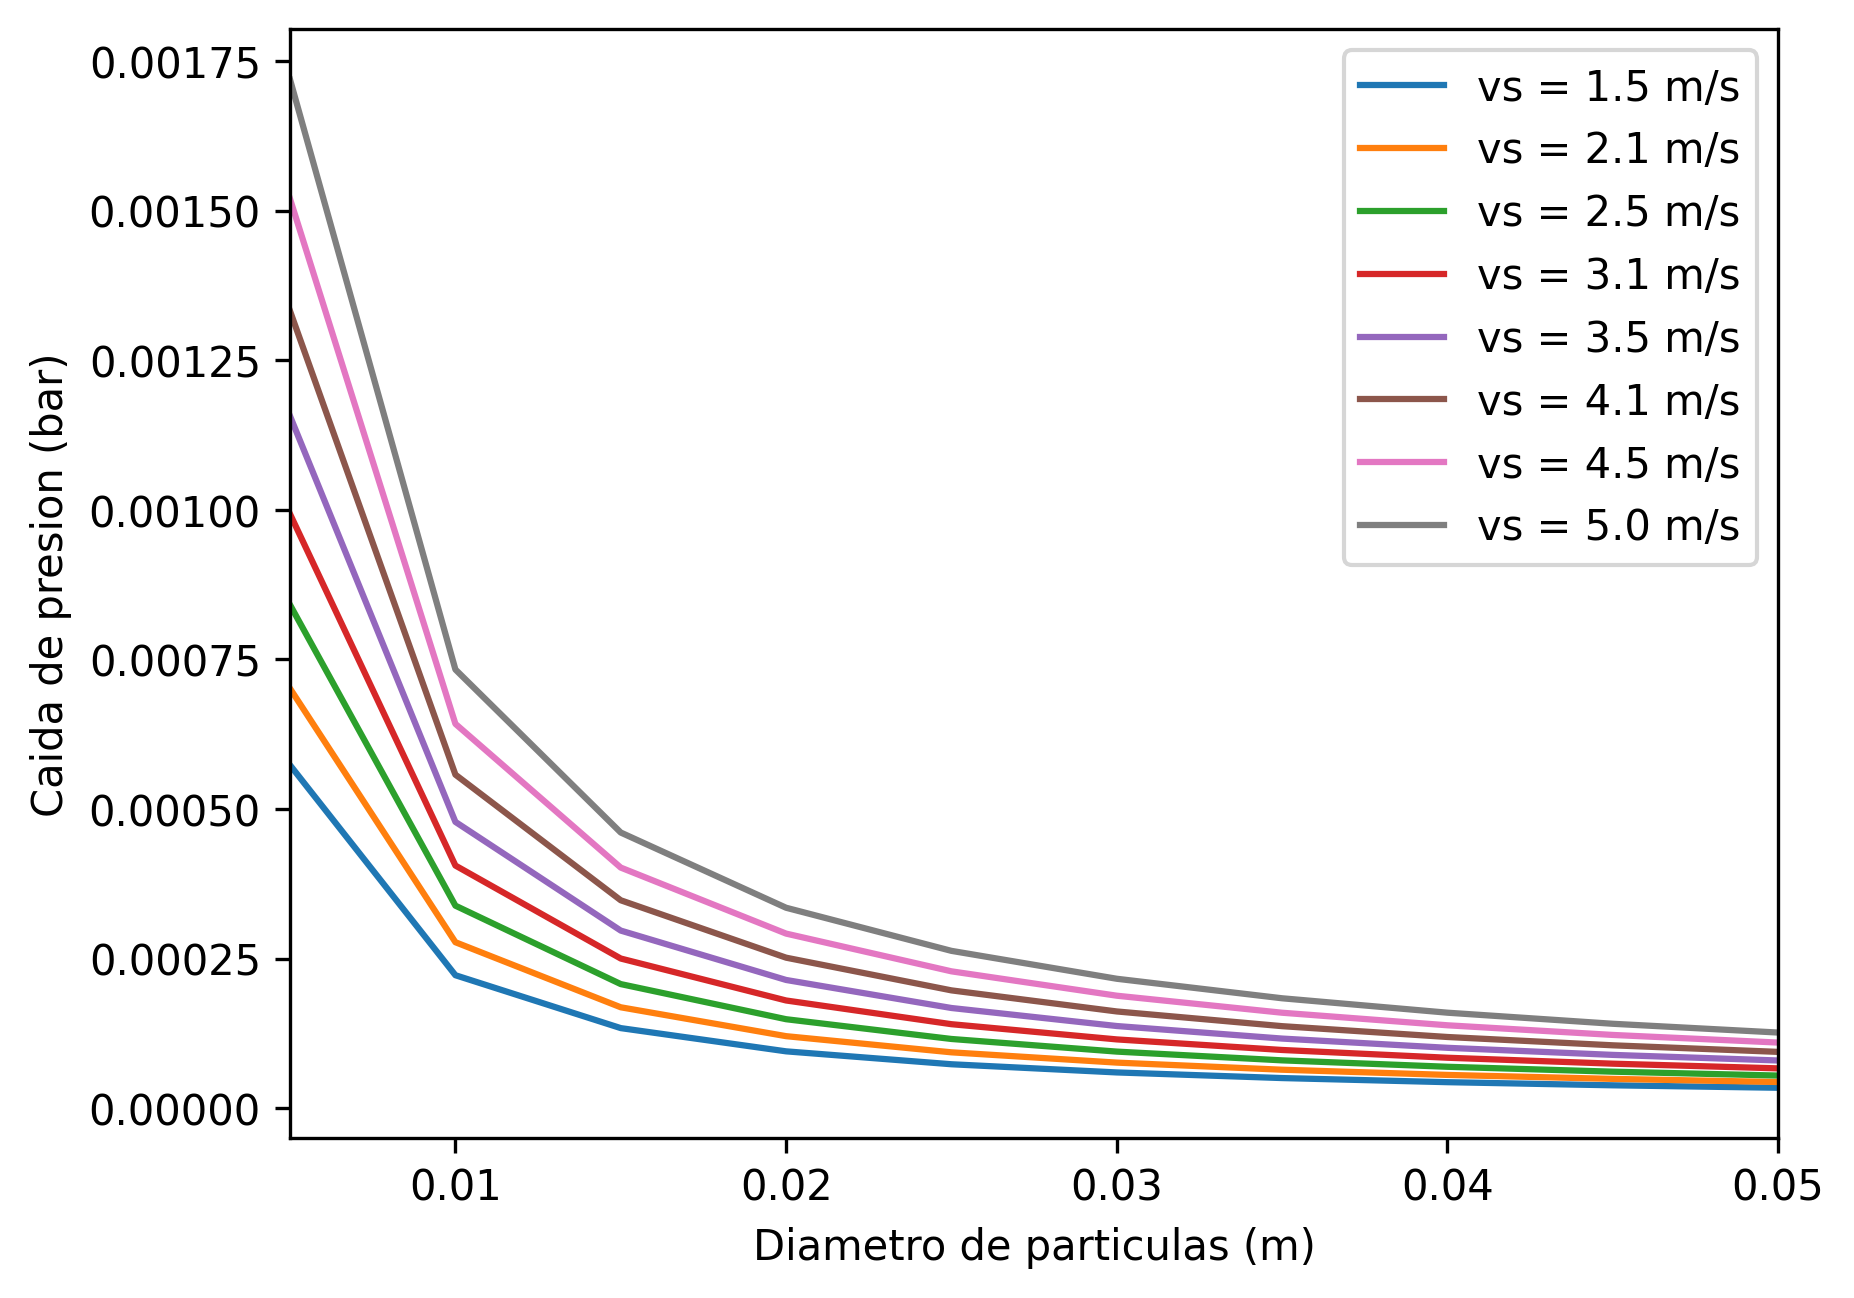
\includegraphics[scale=0.9]{dPrvsDp_03.png}
	\caption{Variación de la caída de presión según el diámetro de la partícula}
\end{figure}
Cada linea del grafico anterior corresponde a una velocidad del flujo del aire, se puede observar como la caída de presión aumenta con partículas mas pequeñas y va disminuyendo conforme crece su tamaño. Por lo tanto, el se requeriría menos energía para empujar el aire entre partículas mas grandes que no oponen menos resistencia al flujo del aire. 
%-----------------------------------------------------------------------
\newpage
\printbibliography
%------------------------------------------------------------------------%
\end{document}
 